% This file was created by tikzplotlib v0.9.2.
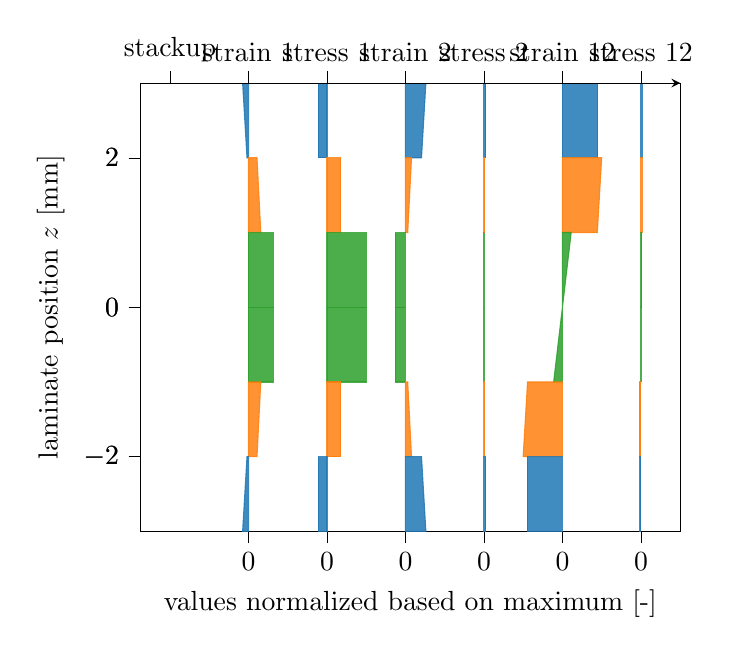
\begin{tikzpicture}

\definecolor{color0}{rgb}{0.12156862745098,0.466666666666667,0.705882352941177}
\definecolor{color1}{rgb}{1,0.498039215686275,0.0549019607843137}
\definecolor{color2}{rgb}{0.172549019607843,0.627450980392157,0.172549019607843}

\begin{axis}[
tick align=outside,
tick pos=left,
x grid style={white!69.0196078431373!black},
xlabel={values normalized based on maximum [-]},
xmin=-0.75, xmax=13,
xtick style={color=black},
xtick={2,4,6,8,10,12},
xticklabels={0,0,0,0,0,0},
y grid style={white!69.0196078431373!black},
ylabel={laminate position \(\displaystyle z\) [mm]},
ymin=-3, ymax=3,
ytick style={color=black}
]
\path [draw=color0, fill=color0, opacity=0.85]
(axis cs:1.85196864675475,3)
--(axis cs:2,3)
--(axis cs:2,2)
--(axis cs:1.96334975975981,2)
--cycle;
\path [draw=color0, fill=color0, opacity=0.85]
(axis cs:3.77807837068539,3)
--(axis cs:4,3)
--(axis cs:4,2)
--(axis cs:3.77807837068539,2)
--cycle;
\path [draw=color0, fill=color0, opacity=0.85]
(axis cs:6,3)
--(axis cs:6.5202553247851,3)
--(axis cs:6.40887421178004,2)
--(axis cs:6,2)
--cycle;
\path [draw=color0, fill=color0, opacity=0.85]
(axis cs:8,3)
--(axis cs:8.04698539145953,3)
--(axis cs:8.04698539145953,2)
--(axis cs:8,2)
--cycle;
\path [draw=color0, fill=color0, opacity=0.85]
(axis cs:10,3)
--(axis cs:10.8974768760748,3)
--(axis cs:10.8974768760748,2)
--(axis cs:10,2)
--cycle;
\path [draw=color0, fill=color0, opacity=0.85]
(axis cs:12,3)
--(axis cs:12.0327682762905,3)
--(axis cs:12.0327682762905,2)
--(axis cs:12,2)
--cycle;
\path [draw=color1, fill=color1, opacity=0.85]
(axis cs:2,2)
--(axis cs:2.2175634580603,2)
--(axis cs:2.31402233142446,1)
--(axis cs:2,1)
--cycle;
\path [draw=color1, fill=color1, opacity=0.85]
(axis cs:4,2)
--(axis cs:4.34869863621424,2)
--(axis cs:4.34869863621424,1)
--(axis cs:4,1)
--cycle;
\path [draw=color1, fill=color1, opacity=0.85]
(axis cs:6,2)
--(axis cs:6.15466051347955,2)
--(axis cs:6.05820164011539,1)
--(axis cs:6,1)
--cycle;
\path [draw=color1, fill=color1, opacity=0.85]
(axis cs:8,2)
--(axis cs:8.02038052887792,2)
--(axis cs:8.02038052887792,1)
--(axis cs:8,1)
--cycle;
\path [draw=color1, fill=color1, opacity=0.85]
(axis cs:10,2)
--(axis cs:11,2)
--(axis cs:10.8886188869949,1)
--(axis cs:10,1)
--cycle;
\path [draw=color1, fill=color1, opacity=0.85]
(axis cs:12,2)
--(axis cs:12.0365115549648,2)
--(axis cs:12.0365115549648,1)
--(axis cs:12,1)
--cycle;
\path [draw=color2, fill=color2, opacity=0.85]
(axis cs:2,1)
--(axis cs:2.63485042380733,1)
--(axis cs:2.63485042380733,0)
--(axis cs:2,0)
--cycle;
\path [draw=color2, fill=color2, opacity=0.85]
(axis cs:4,1)
--(axis cs:5,1)
--(axis cs:5,0)
--(axis cs:4,0)
--cycle;
\path [draw=color2, fill=color2, opacity=0.85]
(axis cs:5.73737354773252,1)
--(axis cs:6,1)
--(axis cs:6,0)
--(axis cs:5.73737354773252,0)
--cycle;
\path [draw=color2, fill=color2, opacity=0.85]
(axis cs:7.99001395353962,1)
--(axis cs:8,1)
--(axis cs:8,0)
--(axis cs:7.99001395353962,0)
--cycle;
\path [draw=color2, fill=color2, opacity=0.85]
(axis cs:10,1)
--(axis cs:10.2227622260101,1)
--(axis cs:10,0)
--(axis cs:10,0)
--cycle;
\path [draw=color2, fill=color2, opacity=0.85]
(axis cs:12,1)
--(axis cs:12.0081333952591,1)
--(axis cs:12.0081333952591,0)
--(axis cs:12,0)
--cycle;
\path [draw=color2, fill=color2, opacity=0.85]
(axis cs:2.63485042380733,0)
--(axis cs:2,0)
--(axis cs:2,-1)
--(axis cs:2.63485042380733,-1)
--cycle;
\path [draw=color2, fill=color2, opacity=0.85]
(axis cs:4,0)
--(axis cs:5,0)
--(axis cs:5,-1)
--(axis cs:4,-1)
--cycle;
\path [draw=color2, fill=color2, opacity=0.85]
(axis cs:6,0)
--(axis cs:5.73737354773252,0)
--(axis cs:5.73737354773252,-1)
--(axis cs:6,-1)
--cycle;
\path [draw=color2, fill=color2, opacity=0.85]
(axis cs:7.99001395353962,0)
--(axis cs:8,0)
--(axis cs:8,-1)
--(axis cs:7.99001395353962,-1)
--cycle;
\path [draw=color2, fill=color2, opacity=0.85]
(axis cs:10,0)
--(axis cs:10,0)
--(axis cs:9.77723777398989,-1)
--(axis cs:10,-1)
--cycle;
\path [draw=color2, fill=color2, opacity=0.85]
(axis cs:11.9918666047409,0)
--(axis cs:12,0)
--(axis cs:12,-1)
--(axis cs:11.9918666047409,-1)
--cycle;
\path [draw=color1, fill=color1, opacity=0.85]
(axis cs:2.31402233142446,-1)
--(axis cs:2,-1)
--(axis cs:2,-2)
--(axis cs:2.2175634580603,-2)
--cycle;
\path [draw=color1, fill=color1, opacity=0.85]
(axis cs:4,-1)
--(axis cs:4.34869863621424,-1)
--(axis cs:4.34869863621424,-2)
--(axis cs:4,-2)
--cycle;
\path [draw=color1, fill=color1, opacity=0.85]
(axis cs:6.05820164011539,-1)
--(axis cs:6,-1)
--(axis cs:6,-2)
--(axis cs:6.15466051347955,-2)
--cycle;
\path [draw=color1, fill=color1, opacity=0.85]
(axis cs:8,-1)
--(axis cs:8.02038052887792,-1)
--(axis cs:8.02038052887792,-2)
--(axis cs:8,-2)
--cycle;
\path [draw=color1, fill=color1, opacity=0.85]
(axis cs:10,-1)
--(axis cs:9.11138111300506,-1)
--(axis cs:9,-2)
--(axis cs:10,-2)
--cycle;
\path [draw=color1, fill=color1, opacity=0.85]
(axis cs:11.9634884450352,-1)
--(axis cs:12,-1)
--(axis cs:12,-2)
--(axis cs:11.9634884450352,-2)
--cycle;
\path [draw=color0, fill=color0, opacity=0.85]
(axis cs:2,-2)
--(axis cs:1.96334975975981,-2)
--(axis cs:1.85196864675475,-3)
--(axis cs:2,-3)
--cycle;
\path [draw=color0, fill=color0, opacity=0.85]
(axis cs:3.77807837068539,-2)
--(axis cs:4,-2)
--(axis cs:4,-3)
--(axis cs:3.77807837068539,-3)
--cycle;
\path [draw=color0, fill=color0, opacity=0.85]
(axis cs:6.40887421178004,-2)
--(axis cs:6,-2)
--(axis cs:6,-3)
--(axis cs:6.5202553247851,-3)
--cycle;
\path [draw=color0, fill=color0, opacity=0.85]
(axis cs:8,-2)
--(axis cs:8.04698539145953,-2)
--(axis cs:8.04698539145953,-3)
--(axis cs:8,-3)
--cycle;
\path [draw=color0, fill=color0, opacity=0.85]
(axis cs:10,-2)
--(axis cs:9.10252312392519,-2)
--(axis cs:9.10252312392519,-3)
--(axis cs:10,-3)
--cycle;
\path [draw=color0, fill=color0, opacity=0.85]
(axis cs:11.9672317237095,-2)
--(axis cs:12,-2)
--(axis cs:12,-3)
--(axis cs:11.9672317237095,-3)
--cycle;
\end{axis}

\begin{axis}[
axis x line=top,
legend cell align={left},
legend style={fill opacity=0.8, draw opacity=1, text opacity=1, at={(1.05,0.5)}, anchor=west, draw=none},
tick align=outside,
x grid style={white!69.0196078431373!black},
xmin=-0.75, xmax=13,
xtick pos=right,
xtick style={color=black},
xtick={0,2,4,6,8,10,12},
xticklabels={stackup,strain 1,stress 1,strain 2,stress 2,strain 12,stress 12},
y grid style={white!69.0196078431373!black},
ymin=-3, ymax=3,
ytick pos=left,
ytick style={color=black}
]
\end{axis}

\end{tikzpicture}
